\clearpage\subsection{Polynomial Asymptotes}
Polynomial asymptotes, unlike vertical and horizontal, are quite tricky. They only occur when the degree of the polynomial in the numerator is greater than that in the denominator. It's not easy to define them using a domain and range because they don't conform strictly to the domain (vertical asymptote) or range (horizontal asymptote). We must, instead, be a little more creative.

Let's remember what division does to a number. Take something like this, for example: $10 \div 3$. In many cases, the number you're dividing by, the divisor, doesn't fit evenly into the number you're dividing, the dividend. In such cases, you are left with a remainder that can be written as a fraction, like so:
\[
3 + \frac{1}{3} \text{.}
\]
The answer we get is such that multiplying it by $3$ gets us back to the original number, $10$. This is true with polynomials, too.

If we allow the following to be true: \\
$f(x)$ - Dividend\\
$g(x)$ - Divisor\\
$q(x)$ - Quotient\\
$r(x)$ - Remainder

Then we can say that the solution to polynomial long division can be expressed like so:
\[
\frac{f(x)}{g(x)} = q(x) + \frac{r(x)}{g(x)}
\]
\clearpage
If we let:\\
$f(x) = x^2$ \\
$g(x) = x + 1$

We get the following solution:
\[
\begin{array}{r|rrrrr}
& x & -1 & &\\ \cline{2-4}
x + 1 & x^2 & 0\\
& -(x^2 & x) & & \\ \cline{2-3}
& & -x & 0\\ 
& & -(-x & -1) \\ \cline{3-5}
& & & 1
\end{array}
\]
In this case, $q(x) = x - 1$ and $r(x) = 1$. Thus, we can write the solution
\[
\frac{x^2}{x + 1} = x - 1 + \frac{1}{x + 1} \text{.}
\]
Notice how, in the $\dfrac{r(x)}{g(x)}$ term, the $x$ is in the denominator. As $x$ grows larger and larger, like to $10000$ or $\infty$, that term becomes smaller and smaller.
\[
    \frac{\text{small number}}{\text{big number}} = \text{small number}
\]
As that term reaches $0$, we are left with $q(x)$, which we established will never actually reach the rational function defined as $\dfrac{f(x)}{g(x)}$. So, no matter what values of $x$ we put in there, and no matter how close $q(x)$ might get to $\dfrac{f(x)}{g(x)}$, it will never touch it. \textbf{That is the definition of an asymptote.}

\begin{definition} % Customized Theorem Envirnment
    Given a dividend, $f(x)$, and a divisor of a lower degree, $g(x)$, written as a rational function, $y = \dfrac{f(x)}{g(x)}$, the polynomial asymptote is defined as 
    \[
        y = q(x) \text{,}
    \]
     where $q(x)$ is the quotient obtained from dividing $\dfrac{f(x)}{g(x)}$.
\end{definition}
\clearpage
While this is true for all rational functions with polynomials in the numerator and denominator, the one you'll most commonly see is a rational function where the degree of the numerator is $1$ greater than the denominator. This is also called a \textbf{slant} or \textbf{oblique} asymptote.

Let's look at a practice problem together.
\begin{problem}
    Find all the asymptotes for the rational function
    \[
        f(x) = \frac{3x^2 + x - 10}{x - 5} \text{.}
    \]
    \textit{Note that $f(x)$, in this case, is the entire rational function and \textbf{not} the dividend.}
\end{problem}

\begin{solution}
    We need to find the quotient of this rational function. Beacuse the denominator has a degree of $1$, we can use synthetic division.
    \[
    \begin{aligned}
        \begin{array}{r|rrr}
            5 & 3 & 1  & -10 \\
            &   & 15 & 90  \\ \cline{2-4}
            & 3 & 16 & 80
        \end{array} \\
        q(x) = 3x + 16
    \end{aligned}
    \]
    That's the first asymptote. There is a second hiding in the denominator. If we set that equal to $0$, we can solve for a vertical asymptote as well.
    \[
        x - 5 = 0 \Longrightarrow x = 5
    \]
    \begin{center}
        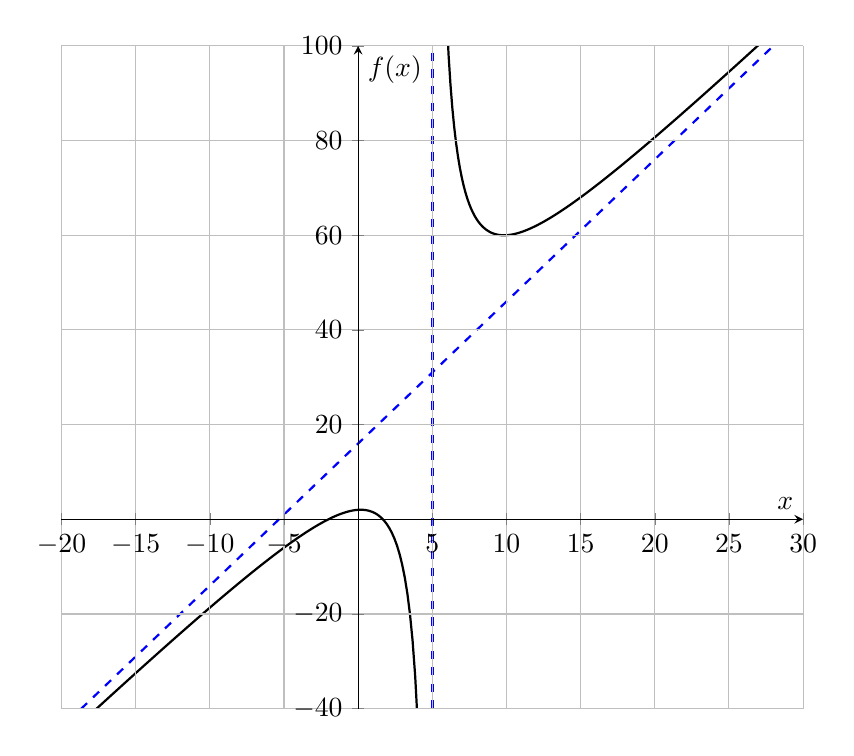
\begin{tikzpicture}
            \begin{axis}[
                axis lines = middle,
                xlabel = $x$, ylabel = {$f(x)$},
                xmin = -20, xmax = 30,
                ymin = -40, ymax = 100,
                grid = both,
                width = 11cm,
                height = 10cm,
                axis on top,
            ]
            % Left branch (x < 5)
            \addplot[black, thick, domain=-30:4.9, samples=200, restrict y to domain=-44:5] 
                {(3*x^2 + x - 10)/(x-5)};
            % Right branch (x > 5)
            \addplot[black, thick, domain=5.1:30, samples=200, restrict y to domain=55:106] 
                {(3*x^2 + x - 10)/(x-5)};
            % Slant asymptote y = 3x + 16
            \addplot[blue, dashed, thick, domain=-30:30, samples=10] {3*x + 16};
            \draw[dashed, blue, very thick] (axis cs:5,\pgfkeysvalueof{/pgfplots/ymin}) -- (axis cs:5,\pgfkeysvalueof{/pgfplots/ymax});
            \end{axis}
        \end{tikzpicture}
    \end{center}
\end{solution}
